% Compile this file with pdflatex to create the list
% of cited papers in the aux file: 'pdflatex latex-examples'
% Then compile the aux file with bibtex to extract the information
% about the cited papers from your bibtex-database: 'bibtex latex-examples'.
% Then you must recompile the tex file with pdflatex to add the list of
% references to the pdf file.
% Because the bibliography is only included in the end of the tex file
% pdflatex did not know the number of each citation during the last
% compilation and therefore added only '[?]' where you cited something.
% You have to compile it once more to finish the pdf document.

\documentclass[runningheads]{llncs}

\usepackage{algorithm}
\usepackage[noend]{algpseudocode}
\usepackage[pdftex]{graphicx}
\usepackage[plainpages=false, pdfpagelabels, bookmarks,  colorlinks=false, % Hyperlinks in PDF output mit blauen Rahmen
               linkbordercolor={0 0 1}, filebordercolor={0 0 1}, citebordercolor={0 0 1},
              menubordercolor={0 0 1}, urlbordercolor={0 0 1}]{hyperref}
\usepackage{booktabs}
\usepackage[utf8]{inputenc}

\title{Seminar Predictive Analytics in Big Data WS 2016/17}
\author{Jasim Waheed Ansari}
\institute{RWTH Aachen University, 52056 Aachen, Germany\\
	jasim.waheed@rwth-aachen.de}

\begin{document}


\maketitle

\begin{abstract}
Predictive Analytics (PA) has replaced the idea of ad-hoc data analysis by fact based decisioning. PA include statistical methods from machine learning and data mining to build data model for regression, prediction, neural networks, classification purposes. In order to incorporate big data criterion, the frameworks and tools that perform modeling using previously stated methods has to address the 4Vs of Big Data, namely volume, veracity, velocity and value. This paper is aimed at providing an overview of big data analytics framework and then highlighting few major tools, comparison and assessment of their characteristics. The second aim is to go through the major issues and challenges that are faced while carrying out PA in big data. We will also address the possible solutions in form of best practices concerning those problems. The third aim is to provide an example from ERP systems to highlight its predictive analytics capabilities using big data systems. The fourth aim is to present a conceptual framework of integrating Complex Event Processing and PA called Predictive Complex Event Processing. We will observe that the given framework would be a generic design pattern for future work. On an ending note, we will demonstrate a case study to get a lucid idea on a practical level.
\end{abstract}

\section{Introduction}
In recent years, there is a flood of data that is shared or generated from various sources. This data is usually presented in an unstructured format such as videos, audios, texts, images. The presented data could or could not be related to each other or there could be a possibility of having some hidden patterns. To perform any sort of analysis, analysts cannot use such unstructured data directly. Such data requires conversion into a well-formed format (similar to a relational data), which could be used by data scientists for purpose of analysis on them. As a result, this structured data can then be used to decipher hidden meanings or pattern which supports prediction of market behavior, enterprise needs, enabling precision based decisioning using technique called Predictive Analytics.
\subsection{What is Predictive Analytics?}
Predictive Analytics is the process of predicting useful information from a set of data (structured,unstructured or semi-structured).
It surrounds techniques from statistics, data mining, machine learning and artificial intelligence.\vspace{-2mm}

\subsubsection{Predictive Analytics steps:}As per general guideline, the steps along with percentage of time spent on each of the step are as follows: \newline
\begin{enumerate}
	\item Understanding the domain (5-10 percent)
	\item Understanding the data (5-10 percent)
	\item Preparing the data (50-60 percent)
	\item Modeling (5-15 percent)
	\item Evaluation (5-10 percent)
	\item Deployment (10-15 percent)
\end{enumerate} 
It is worth noting that each step could have as many iterations as needed. Adding to that, core effort in processing is emphasized at the data.\newline
Figure \ref{fig:Figure1} shows Predictive Analytics process which is followed actively by analysts across various industries \cite{6}
\begin{figure}[htbp]
	% center the image.
	\centering
	
	% include a png file. Adapt size to 0.5 * textwidth and retain aspect ratio (!)
%	\resizebox{\textwidth}{!}{Figure1.png}}
	% NOTE: if possible do not include bitmap graphics in your paper, if available use
	% a vector graphics format
	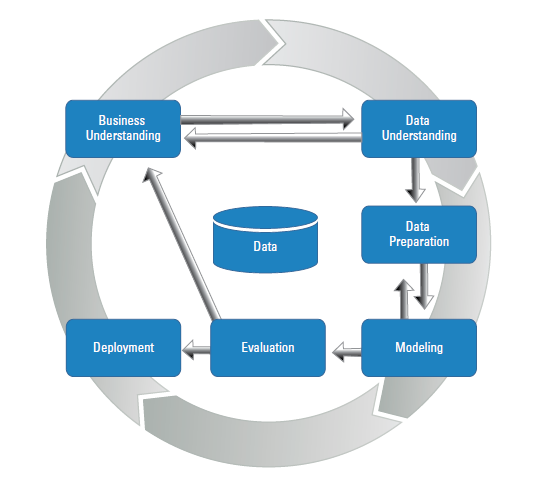
\includegraphics[scale=0.7]{Figure1.png}
	\caption{Predictive analytics process}
	\label{fig:Figure1}
\end{figure}
\newline
\subsubsection{Techniques available:}
From predictive analytics process, modeling and evaluation steps are where analysts use algorithms to produce key information they desire. Predictive modeling algorithms \cite{7} falls under Supervised Learning. In Supervised Learning, the predictor value or target variable is \textit{supervisor}, it is the column in dataset that is used for predicting value from other column values. It is divided into two sets:
\begin{enumerate}
	\item Classification: class based or discrete target variable
	\item Regression: continuous target variable 
\end{enumerate} 
Figure \ref{fig:Figure2} shows Predictive Analytics techniques used for modeling\cite{8}.
\begin{figure}[htbp]
	% center the image.
	\centering
	
	% include a png file. Adapt size to 0.5 * textwidth and retain aspect ratio (!)
	%	\resizebox{\textwidth}{!}{Figure1.png}}
	% NOTE: if possible do not include bitmap graphics in your paper, if available use
	% a vector graphics format
	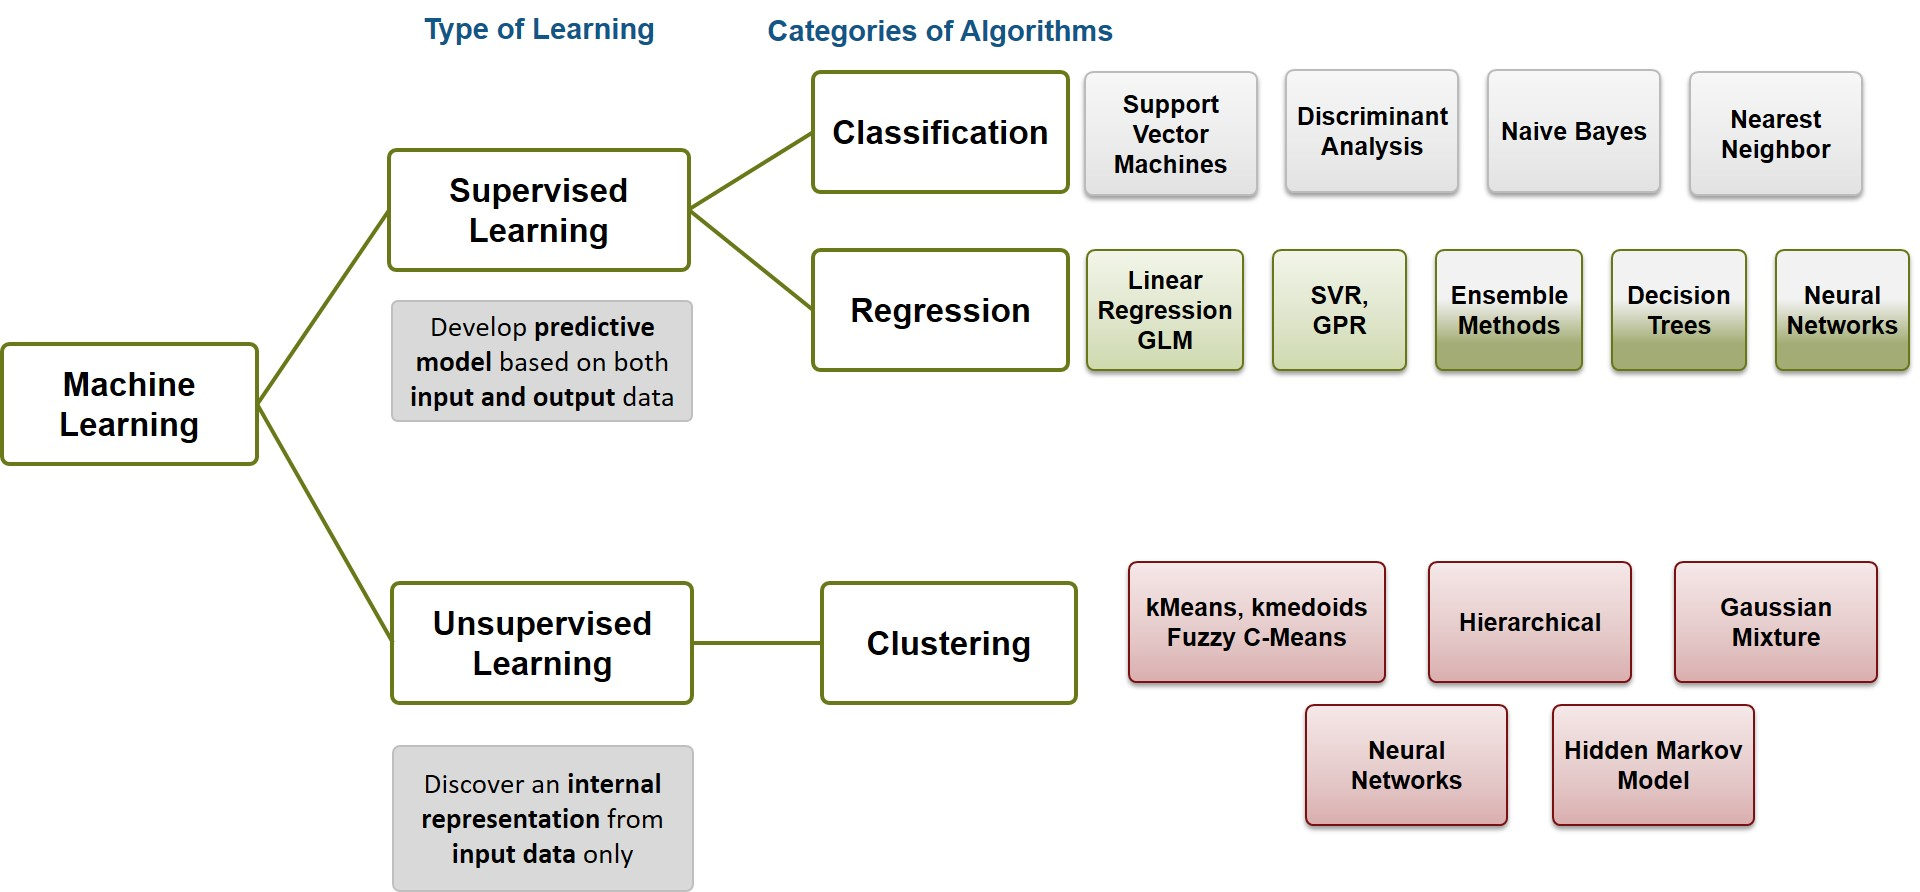
\includegraphics[scale=0.35]{Figure2.jpg}
	\caption{Predictive analytics techniques}
	\label{fig:Figure2}
	
\end{figure}

\vspace{-4mm}
\subsection{Predictive Analytics: Harness the power of Big Data}Almost every decision making process, be it in any enterprise, involves predictive analytics to drive their business better and helps gaining competitive edge in the market. Decision making in current era is based on day-to-day operational business data rather than on only special projects or scenario. Current tools and technologies are unsatisfactory and not up to standards to process such huge chunks of operational data. They are also unable to make in-depth insight and generate value. \newline
Thanks to Big Data technology and tools, predictive analytics can be applied to deluge of data at enterprise level, sometimes also called as Big Data Analytics. We have now many ways to tackle and test different predictive models at various level of framework for business strategies. Figure \ref{fig:Figure3} shows delineation of characteristics of Predictive Analytics techniques in transactional databases vs big data technologies. The former is based on prediction through historical structured data whereas big data platform can be used for modeling in real-time with structured, unstructured or semi-structured data. The common methods involved in transactional databases are data mining algorithms such as decision trees, regression, clustering, association rules, etc. In big data mediums, advanced techniques such as speech recognition, mobile based analytics, etc. [\cite{7}].\\
In the upcoming sections, we will be providing the conjunction of Predictive Analytics with Big Data technology and bring the following topics in coherence:\newline
(1) understanding big data architecture for analytical perspective \newline
(2) comparison and assessment of big data analytical tools used for predictions \newline
(3) address few of the challenges which collides interest of predictive analytics with big data. One of the key challenges being privacy- arising from ever increasing data from online services and personal devices such as mobile phones. These are subjected to risk of personal information being exposed for illicit uses. \newline
(4) discuss example from Enterprise Resource Planning (ERP) systems, and explore the opportunities of predictive analytics on ERP system's integrated big data hub. \newline
(5) discuss about Complex Event Processing which deals in identifying complex events based on the rules dictated by users of the system. In order to avoid the manual intervention of users for providing progressive rules, we will discuss about the framework that includes Predictive Analytics technologies in Complex Event Processing tools and applications. \newline
(6) case study demonstrating the power of predictive analytics coupled with big data technology.
\begin{figure}[htbp]
	% center the image.
	\centering
	\vspace{-0.5em}
	% include a png file. Adapt size to 0.5 * textwidth and retain aspect ratio (!)
	%	\resizebox{\textwidth}{!}{Figure1.png}}
	% NOTE: if possible do not include bitmap graphics in your paper, if available use
	% a vector graphics format
	\hspace*{-0.45cm}
	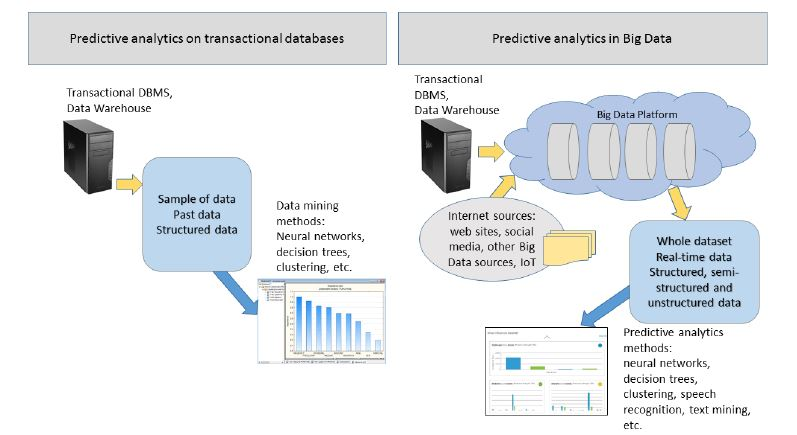
\includegraphics[scale=0.6]{Figure3.jpg}
	\caption{Predictive analytics in traditional databases vs Big Data}
	\label{fig:Figure3}
	\vspace{-0.5em}
\end{figure}
\section{Big Data System Architecture}
A big data system is immensely complex. In order to demonstrate the architecture of predictive analytics in big data, we should firstly understand the categorization of two paradigms of big data analytics with respect to processing time requirements:
\begin{itemize}
	\item Stream Processing: Streaming processing data is dependent on fresh data i.e. it needs to be analyzed as soon as it is available. Some famous open source systems available are Storm and Kafka.
	\item Batch Processing: In batch processing, data is stored as chunk and then analyzed. One of the most famous models available is Map Reduce.
\end{itemize}
In this section, we will discuss architecture based on batch processing types, since it is widely adopted in industries. We will show one such framework placed on value chain for big data analytics\cite{5}. Big data value chain framework involves four stages i.e. generation, acquisition, storage and analytics. In this work, we will see leading technologies in analysis phase.
\subsection{Big Data Value Chain architecture}
This architecture is based on system engineering approach, well recognized in industries, the notion is to break down the big-data system into four continuous phases in horizontal axis as shown in Figure \ref{fig:Figure4} \cite{5}.
\paragraph{Data Analysis:} It is the main and concluding step from big data value chain that focuses on the aspect of analytics. This phase supports mechanisms or tools to investigate, transform, and modeling data to discover insights. We will discuss hereby some classification metric of big data analytics. Furthermore, we will describe common methods in big data analytics that together build the pillar for making predictions comprehensively. We will then give an overview picture of nomenclature of big data analytics with respect to data type.
\subsubsection{Categories:}
Blackett et al \cite{10} proposed classification of big data analytics into three levels as follows:
\begin{enumerate}
	\item Descriptive Analytics: analyses historical dataset to describe what happened. It is widely used with business intelligence or ERP solutions.
	\item Predictive Analytics: focuses on future predictions and trends, uses supervised learning algorithms to understand trends, and data mining exacts insight.
	\item Prescriptive Analytics: focuses on decision making. For instance, simulation is used to analyze the systems and recognize various optimization techniques to get efficient solutions.
\end{enumerate} 

\begin{figure}[htbp]
	% center the image.
	\centering
	\vspace{-0.85cm}
	% include a png file. Adapt size to 0.5 * textwidth and retain aspect ratio (!)
	%	\resizebox{\textwidth}{!}{Figure1.png}}
	% NOTE: if possible do not include bitmap graphics in your paper, if available use
	% a vector graphics format
	\hspace*{-0.45cm}
	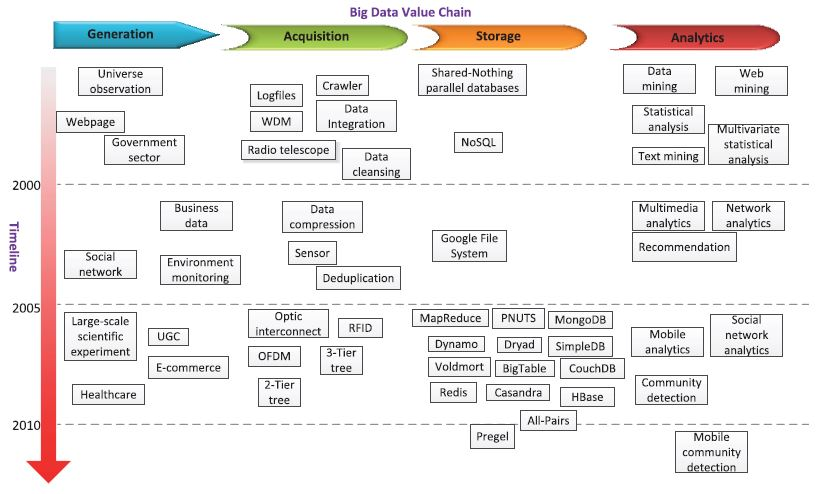
\includegraphics[scale=0.6]{Figure4.jpg}
	\caption{Big data value chain architecture. Horizontal axis composes of four continuous phases for data life cycle. For each stage, we demonstrate cutting edge technologies available past ten years in vertical axis}
	\label{fig:Figure4}
	\vspace{-0.5em}
\end{figure}
\section{Predictive Analytics Technologies}
The technology that is adept in supporting big data includes  new kinds of database platforms(for example, Hadoop and Spark) as a central core of big data systems, predictive tools are built on top of them to perform analytics in cloud, thus enabling enterprises with scalability and on-demand usage. We will see software stacks as framework for predictive analytics in Hadoop and Spark respectively.
\subsection{Hadoop Software Stack}
It is a massive framework encompassing different modules, including Hadoop Distributed File System (HDFS) \& Hbase for data storage, MapReduce as computation core for analysis on data, Flume \&  Sqoop as integration tools. This framework is in accordance with big data value chain architecture and it is used as a powerful solution for batch-type processing applications. The layered core software libraries is shown in figure \ref{fig:Figure4}. On top of this framework is the data mining library called \textit{Mahout}. \subsubsection{Mahout:}It contains major algorithms responsible for clustering, classification and recommendation (collaborative filtering) to support large-scale predictive analytics model. One of the most famous ways to operate on data needed for such a model is to deploy Mahout in machine that is already executing Hadoop\cite{12}. Hadoop nominates a master system coordinates with the other systems (i.e. Map systems and Reduce systems) applied in its distributed processing.

\begin{figure}[htbp]
	% center the image.
	\centering
	\vspace{0.85cm}
	% include a png file. Adapt size to 0.5 * textwidth and retain aspect ratio (!)
	%	\resizebox{\textwidth}{!}{Figure1.png}}
	% NOTE: if possible do not include bitmap graphics in your paper, if available use
	% a vector graphics format
	\hspace*{-0.45cm}
	
	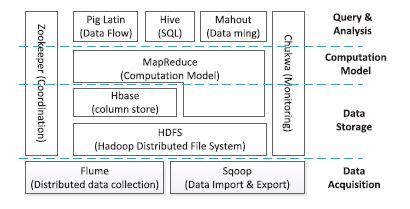
\includegraphics[scale=0.7]{Figure6.jpg}
	\caption{Hadoop Software Stack, covering the major function of big data value chain, inclusive of data import, storage and processing}
	\label{fig:Figure5}
	\vspace{-0.5em}
\end{figure}
\subsection{Spark Framework for real-time analytics}
Another famous open-source platform for processing big data that is best applicable for stream-oriented data processing. Spark is viewed as a strong contender to replace MapReduce capabilities of Hadoop. Spark sits on top of existing Hadoop cluster which relies on YARN for efficient resource management and job scheduling. 
\subsubsection{MLlib:}It is effective for iterative-based large scale machine-learning applications for predictive analytics. The algorithms are written in Scala and the linear algebra libraries uses native C++. MLlib includes support for JAVA, Scala, and Python APIs. They are released as part of Spark project under Apache 2.0. Figure \ref{fig:Figure6} shows Apache Spark ecosystem, where MLlib is built on top of Spark.
\begin{figure}[htbp]
	% center the image.
	\centering
	\vspace{0.85cm}
	% include a png file. Adapt size to 0.5 * textwidth and retain aspect ratio (!)
	%	\resizebox{\textwidth}{!}{Figure1.png}}
	% NOTE: if possible do not include bitmap graphics in your paper, if available use
	% a vector graphics format
	\hspace*{-0.45cm}
	
	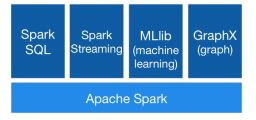
\includegraphics[scale=0.7]{Figure7.jpg}
	\caption{Spark Ecosystem}
	\label{fig:Figure6}
	\vspace{-0.5em}
\end{figure}

\subsection{Big Data Predictive Analytics Tools}
Extremely strong knowledge in statistics and technical skills were previously required to carry out predictive modeling, due to complexities in the usage of statistical models and tools. Advanced abilities were also required in analyzing the result. However, due to the increasing growth of technology the tools are no more focused to advanced experts. Business experts from various organizations can use tools marketed by proprietary software enterprises and open source organizations to predict their business growth.
Figure \ref{fig:Figure7} \cite{14} shows Predictive Analytics tools classification with its characteristics and examples.

\begin{figure}[htbp]
	% center the image.
	\centering
	
	\vspace{-1.5em}
	% include a png file. Adapt size to 0.5 * textwidth and retain aspect ratio (!)
	%	\resizebox{\textwidth}{!}{Figure1.png}}
	% NOTE: if possible do not include bitmap graphics in your paper, if available use
	% a vector graphics format
	\hspace*{-0.45cm}
	
	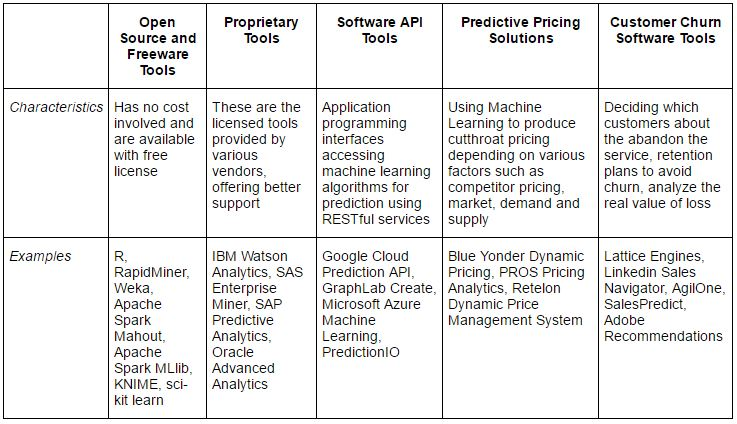
\includegraphics[scale=0.65]{Figure8.jpg}
	\caption{Predictive Analytics Tools Classification and Examples}
	\label{fig:Figure7}
	
\end{figure}
\begin{figure}[htbp]
	% center the image.
	\centering
	
	\vspace{-1.3em}
	% include a png file. Adapt size to 0.5 * textwidth and retain aspect ratio (!)
	%	\resizebox{\textwidth}{!}{Figure1.png}}
	% NOTE: if possible do not include bitmap graphics in your paper, if available use
	% a vector graphics format
	\hspace*{-0.45cm}
	
	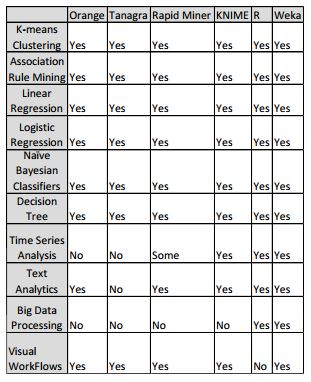
\includegraphics[scale=0.65]{Figure9.jpg}
	\caption{Comparison matrix showing few open source tools supporting common predictive analytics techniques}
	\label{fig:Figure8}
	
\end{figure} 

\vspace{-1.5em}
\subsubsection{Comparison of open source tools}
The comparison matrix\cite{15} in the given figure \ref{fig:Figure8} explains some of the open source tools (described previously) capabilities with respect to data science techniques. It needs to be observed that Weka offers the maximum support on an open-source level. In the later section of this paper, we will highlight the case study of predicting chronic kidney diseases using Weka tool.

\section{Issues in predictive analytics}
Predictive analytics are built on set model solutions, and if these are not optimized and addressed properly, they may present problems such as slow down the progress and alter the business analytics solutions. We will address few of the issues associated in this section.
\begin{itemize}
	\item Data quality: Data is fundamental to predictive analytics, and it is highly recommended to have a deeper knowledge on the available data before investing in any predictive analytics technologies. Andreescu, et al figured out that the poor data could lead to erroneous results. In order to maximize the quality, data should be subjected to data preparation, cleaning and formatting. All of which are significant part of data mining steps.\\
	\item Model complexity: Analytic solutions developed for predictions are generally known for taking overly complex models and delivering easy-to-understand results from them. But, companies get carried away and started to expect much more beyond the tools capabilities. This eventually end up slowing down the delivering of report. To maximize the result while minimizing the time to deliver reports, an effective model life-cycle management approach is needed to be adopted.\\
	\item Communication gap: There may be a gap of conveying the insights from data scientists to business users. In order to overcome such problems, enterprises should have skilled enough people not only in analyzing trend but also in documenting it and presenting this info in crisp and compelling terms.\\
	\item Privacy concerns: This is one of the key issues of all. As the big data continues to grow bigger, the analytical capabilities on them poses severe risk of discovering insights in form of individual data. Therefore, such analytical insight could never rule out to make individual data anonymised. We look into some best practices available for preserving privacy of the user data. 
\end{itemize}
\subsection{Best practices available for preserving privacy}
In this section, we discuss three privacy preservation methods \cite{16}.
\begin{enumerate}
	\item Data Anonymization: It is the process of masking or changing data that will be published in such a way that doesn't conceal sensitive information such as full name, social security number etc. The problem with anonymization is that the sensitive information can still be de-identified through linkability with external sources. Three privacy methods with respect to data anonymization are as follows:
	\subitem K-Anonymity: A dataset is K-Anonymous if for any row in the dataset with given attributes, there exists atleast K-1 similar records. It is achieved by suppression or generalization.
	In suppression, attributes are masked by some constant values 0,* etc.
	In generalization, identifiers are masked by a more generic value from levels up the hierarchy.
	\subitem L-Diversity: It tries to bring diversity in sensitive data record. It maintains that each equivalence class has atleast L disparate values of sensitive columns.
	\subitem T-Closeness: A dataset is T-closed if distance between distribution of sensitive column data in a particular equivalence class and distribution in whole dataset is no more than a threshold value of T.
	\item Notice and Consent: It is one of the most common method for web applications and services. The consumer needs to approve the notice before using the services. It imposes a privacy preservation on the user.
	\item Differential Privacy: It is a method empowering data scientists to extract the overall picture from datasets but holding strong privacy on individual data. In contrast to anonymization, there is no modification done to data but there is an added firewall-like interface above the dataset to calculate the results and add much needed inacurracies.
\end{enumerate}

\section{Example: Big Data Predictive Analytics in ERP Systems}
Enterprise Resource Planning(ERP) systems are business process management software, which integrates applications across different departments of an enterprise to provide a holistic view of employees, which corresponds to financial impact on the business. Adding predictive analytics capabilities to ERP systems render progressive guideline to yield effective informed decision. 
\subsection{Enterprise Platform for Decision Management in ERP System}
Predictive analytics on enterprise level enables unlocking insights from structured and unstructured data, identifying classification, associations, and segmentations. Figure\ref{fig:Figure9} shows deployment of Decision as a Service in ERP system landscape. This framework is potent for transforming large set of transactional data into mathematical form for being usable by predictive models.
\begin{figure}[htbp]
	% center the image.
	\centering
	
	\vspace{-1.3em}
	% include a png file. Adapt size to 0.5 * textwidth and retain aspect ratio (!)
	%	\resizebox{\textwidth}{!}{Figure1.png}}
	% NOTE: if possible do not include bitmap graphics in your paper, if available use
	% a vector graphics format
	\hspace*{-0.45cm}
	
	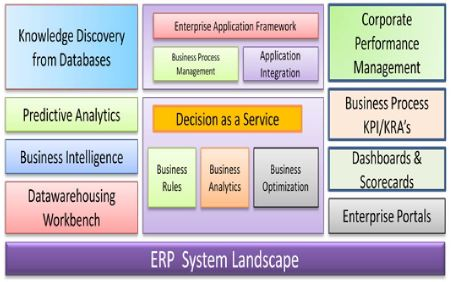
\includegraphics[scale=0.65]{Figure11.jpg}
	\caption{Enterprise Platform for Decision Making \cite{2}}
	\label{fig:Figure9}
	
\end{figure}

\subsection{ERP with Big Data Using Predictive Analytics}
In current business situations, integrating \cite{2} big data solutions to ERP helps in using big data from diverse sources such as web logs, documents, call center transactions, sensors etc.
Figure \ref{fig:figure10} discusses big data predictive analytics framework aimed at automating operational decisioning processes in enterprises using SAP ERP system.
\begin{figure}
	\centering
	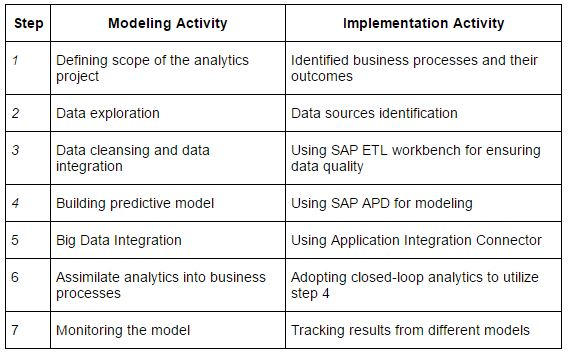
\includegraphics[width=0.7\linewidth]{Figure12}
	\caption{Application Framework for Big Data Predictive Analytics in ERP Systems \cite{2}}
	\label{fig:figure10}
\end{figure}

\subsection{Predictive Analytics steps in ERP systems}
The key factor for performing analytics for prediction is to build a predictive model. Following \ref{fig:figure11} explains the steps involved in model development: 
\begin{figure}
	\centering
	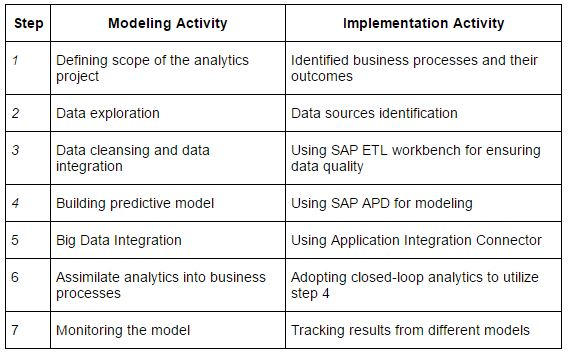
\includegraphics[width=0.7\linewidth]{Figure12.jpg}
	\caption{Model Development Tasks}
	\label{fig:figure11}
\end{figure}
The author emphasizes that decisioning framework for ERP system should be designed to be agile and adaptive. Future work of the explained application framework  is aimed at automating strategical decision making.

\section{Conceptual Framework: Predictive Complex Event for Pro-Active Streaming Applications}
The increasing growth of applications based on streaming data such as Internet of Things(IoT) are gaining popularity for predictive analytics. Data from IoT devices, stock markets for market assessment, credit card fraud detection etc. generated in the form of real-time events, which form complex patterns where such pattern represents a unique event. The need to store, process and analyze these unique events in real-time forms the basis of research area called Complex Event Processing(CEP).
Even though CEP provides power in making decisions from streaming data on reactive basis by using pre-defined rules, but it lacks the capabilities of predictions using historical data i.e. proactive way. The current prediction techniques involved are based on static model parameters, however CEP engines are susceptible to adaptive algorithms depending on environment. Therefore, we firstly describe the authors' proposed framework based on PA and CEP. Later, we explain adaptive prediction algorithm. We conclude it with evaluation using case study from adaptive traffic management system which show accuracy upto 90\%.
 
\subsection{Proposed Architecture}Proposed Architecture is shown in figure \ref{fig:figure12}
\begin{figure}
	\centering
	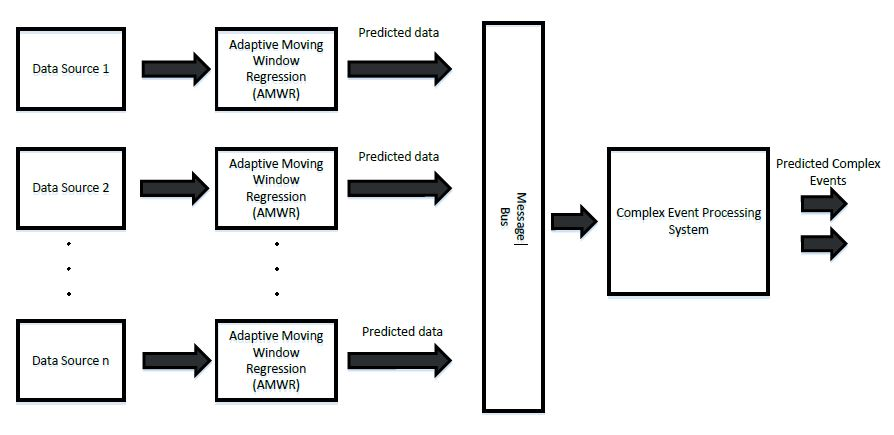
\includegraphics[width=0.8\linewidth]{Figure13.jpg}
	\caption{CEP-PA Conceptual Architecture \cite{17}}
	\label{fig:figure12}
\end{figure}
Different data from sources is accessed from RESTful web services, and then Adaptive Moving Window Regression (AMWR) algorithm is applied. The predicted data produced from the algorithm is published on the message bus, which has a distributed publisher/subscriber architecture and then CEP Engine accesses it.
The different components involved in our proposed architecture is described below.
\subsubsection{A. Adaptive Moving Window Regression(AMWR)} This algorithm handles proactive dynamic IOT data. Generally for statistical data, the predictive model is trained using historical data. Once the model is developed, it cant be changed. However, with changing data and environment the model is prone to damage and adversaries. The author \cite{17} has proposed an approach to retraining the model at regular interval. Three main steps to describe the model is as follows:
\begin{enumerate}
	\item Selection of ML algorithm: We are using Support Vector Regression (SVR) to model multi-valued variable or non-linear data. SVR is an extension of Support Vector Machine (SVM), which maps the training dataset to high-dimensional feature space using kernel function, it fits the training set using hyperplane.
	\item Choice of optimum training window size: The author proposed an algorithm to find the best training window size automatically, so that the error and over-fitting is reduced. The metric to decide the window size is by analyzing Mean Absolute Percentage Error (MAPE). 
	\item Adaptive size for prediction window: The idea is to have an adaptive size for window so that the accuracy and performance of the model is high enough. The algorithm presented by the author is as follows:
\begin{algorithm}
\caption{Adaptive Prediction Window Size}\label{Adaptive Prediction Window Size}
\begin{algorithmic}[1]
	\Procedure{PredictionWindow(x\textsubscript{actual},x\textsubscript{predicted})}{}\\MAPE=mean(abs((x\textsubscript{actual}-x\textsubscript{predicted})/x\textsubscript{actual})*100)\\
	if MAPE \textgreater 20\% then \\
		PredictionWindow = PredictionWindow - 1 \\
	else if MAP \textless 5\% then \\
	PredictionWindow = PredictionWindow + 1 \\
	else\\
	PredictionWindow = PredictionWindow\\
	end if\\
	return PredictionWindow\\
	End procudure
	
\EndProcedure 
\end{algorithmic}
\end{algorithm}


\end{enumerate}


\subsubsection{B. Complex Event Processing} The different components involved in CEP which provides basic operations on the data generated from different sources are:

\begin{enumerate}
\item Filters: Discard or keep the events of interest 
\item Windows: Provides a tool to exact time-related patters from incoming events to dervice complex event
\item Joins: To correlate events coming from different data streams using AND/OR logical operator
\item Aggregations: CEP solutions have simple aggregators such as SUM, MIN, MAX etc. to analyze the events
\end{enumerate}

\subsection{Example: Designing CEP predictive rule for adaptive traffic management} The author has taken the dataset of traffic provided by city of Madrid. The city of Madrid has deployed over a thousand of sensors at fixed locations to monitor the traffic congestion features such as traffic intensity (average number of vehicles per hour) and average traffic speed.
\begin{figure}
	\centering
	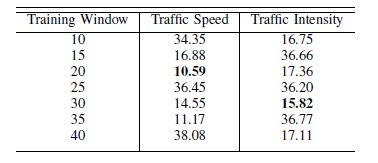
\includegraphics[width=0.8\linewidth]{Figure15.jpg}
	\caption{MAPE \% for traffic speed and intensity \cite{17}}
	\label{fig:figure13}
\end{figure}
 \begin{figure}
	\centering
	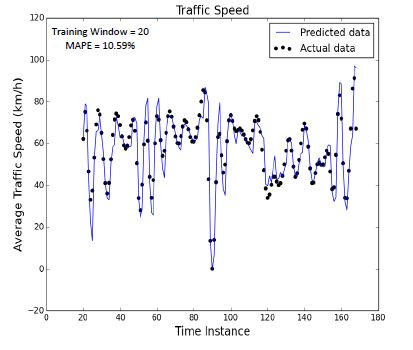
\includegraphics[width=0.8\linewidth]{Figure16.jpg}
	\caption{Prediction result for traffic speed \cite{17}}
	\label{fig:figure14}
\end{figure}
\begin{figure}
	\centering
	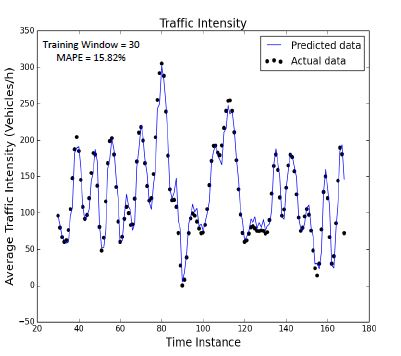
\includegraphics[width=0.8\linewidth]{Figure17.jpg}
	\caption{Prediction result for traffic intensity \cite{17}}
	\label{fig:figure15}
\end{figure}
\subsubsection{Result evaluation} We use our proposed algorithm to predict the traffic in future using the aforementioned two factors. The real time data is available using RESTful web service as XML format. We used the historical data of first few hours to develop an initial model of optimum window size. Table given in figure \ref{fig:figure13} shows the error percentage for various window sizes on traffic speed and intensity. Least error percentage for both of the factor is selected during training phase. Once the initial model is deployed and the stream data is plugged in, the predicted data is compared with actual data. If the error starts to increase then window size is needed to be decreased, which in turn retrains the model to track the actual data.
Figure \ref{fig:figure14} and figure \ref{fig:figure15} explains result of prediction using AMWR algorithm for traffic speed and traffic intensity respectively. We see that this approach results in correctly tracking the predicted data with actual data.
Once the predicted result is available, CEP can be utilized to infer events. The proposed algorithm for CEP rule for this example is as follows: \\
\begin{algorithm} 
	\caption{Example rule for CEP \cite{17}}\label{Example rule for CE}
	\begin{algorithmic}[1]
		\Procedure{CEP(speed,intensity)}{}\\
		for(speed,intensity) TupleWindow(3) do \\
		if (speed(t) \textless speed\textsubscript{threshold} and intensity(t) \textless \
		intensity\textsubscript{threshold} AND \\
	    speed(t + 1) \textless speed(t) and intensity(t + 1) \textless \\
	    intensity(t) AND \\
	    speed(t+2) \textless speed(t+1) and intensity(t+2) \textless \\
        intensity(t + 1)) then \\
		Generate Complex Event "Congestion" \\
		end if
		\EndProcedure 
	\end{algorithmic}
\end{algorithm}
\\It is worth observing that the proposed framework from the use case explained is a promising solution for intelligent transport systems and other applications which are dynamic in nature. 
\section{Conclusion} In this work, a brief study on role of Predictive Analytics has been analyzed in Hadoop and Spark ecosystem, comaprison of various PA tools, the various challenges involved to carry out PA, an example framework from ERP system to get a lucid idea on how the various enterprises(example, SAP) are adopting the big data analytics infrastructure and a conceptual framework to understand the power of PA into event processing engines. 


\bibliographystyle{splncs} % other possible styles: plain, unsrt, abbrv, alpha
\bibliography{Example-Bib}

\end{document}
